%!TEX TS-program = xelatex
%!TEX encoding = UTF-8 Unicode
% Awesome CV LaTeX Template
%
% This template has been downloaded from:
% https://github.com/posquit0/Awesome-CV
%
% Author:
% Claud D. Park <posquit0.bj@gmail.com>
% http://www.posquit0.com
%
% Template license:
% CC BY-SA 4.0 (https://creativecommons.org/licenses/by-sa/4.0/)
%


%%%%%%%%%%%%%%%%%%%%%%%%%%%%%%%%%%%%%%
%     Configuration
%%%%%%%%%%%%%%%%%%%%%%%%%%%%%%%%%%%%%%
%%% Themes: Awesome-CV
\documentclass[11pt, a4paper]{awesome-cv}

%%% Override a directory location for fonts(default: 'fonts/')
\fontdir[fonts/]

%%% Configure a directory location for sections
\newcommand*{\sectiondir}{resume/}

%%% Override color
% Awesome Colors: awesome-emerald, awesome-skyblue, awesome-red, awesome-pink, awesome-orange
%                 awesome-nephritis, awesome-concrete, awesome-darknight
%% Color for highlight
% Define your custom color if you don't like awesome colors
\colorlet{awesome}{awesome-red}
%\definecolor{awesome}{HTML}{CA63A8}
%% Colors for text
%\definecolor{darktext}{HTML}{414141}
%\definecolor{text}{HTML}{414141}
%\definecolor{graytext}{HTML}{414141}
%\definecolor{lighttext}{HTML}{414141}

%%% Override a separator for social informations in header(default: ' | ')
%\headersocialsep[\quad\textbar\quad]


%%%%%%%%%%%%%%%%%%%%%%%%%%%%%%%%%%%%%%
%     3rd party packages
%%%%%%%%%%%%%%%%%%%%%%%%%%%%%%%%%%%%%%
%%% Needed to divide into several files
\usepackage{import}

%%%%%%%%%%%%%%%%%%%%%%%%%%%%%%%%%%%%%%
%     Personal Data
%%%%%%%%%%%%%%%%%%%%%%%%%%%%%%%%%%%%%%
%%% Essentials

\name{Dat-Chanh}{Nguyen}
\address{Luzernerstrasse 71, 6014 Luzern}
\mobile{(+41) 78-653-0756} 
%%% Social
\email{nguyenchanhdat@gmail.com}
%\homepage{www.posquit0.com}
\github{gipfeli}
\linkedin{gipfeli}
\stackoverflow{1763783}{gipfeli}
%%% Optionals
%\position{Werkstudent im Bereich Gas Sensors}
%\quote{``Make the change that you want to see in the world."}


%-------------------------------------------------------------------------------
\begin{document}
\begin{minipage}{0.8\textwidth}
% Print the header with above personal informations
\makecvheader
\end{minipage}
\begin{minipage}{0.15\textwidth}
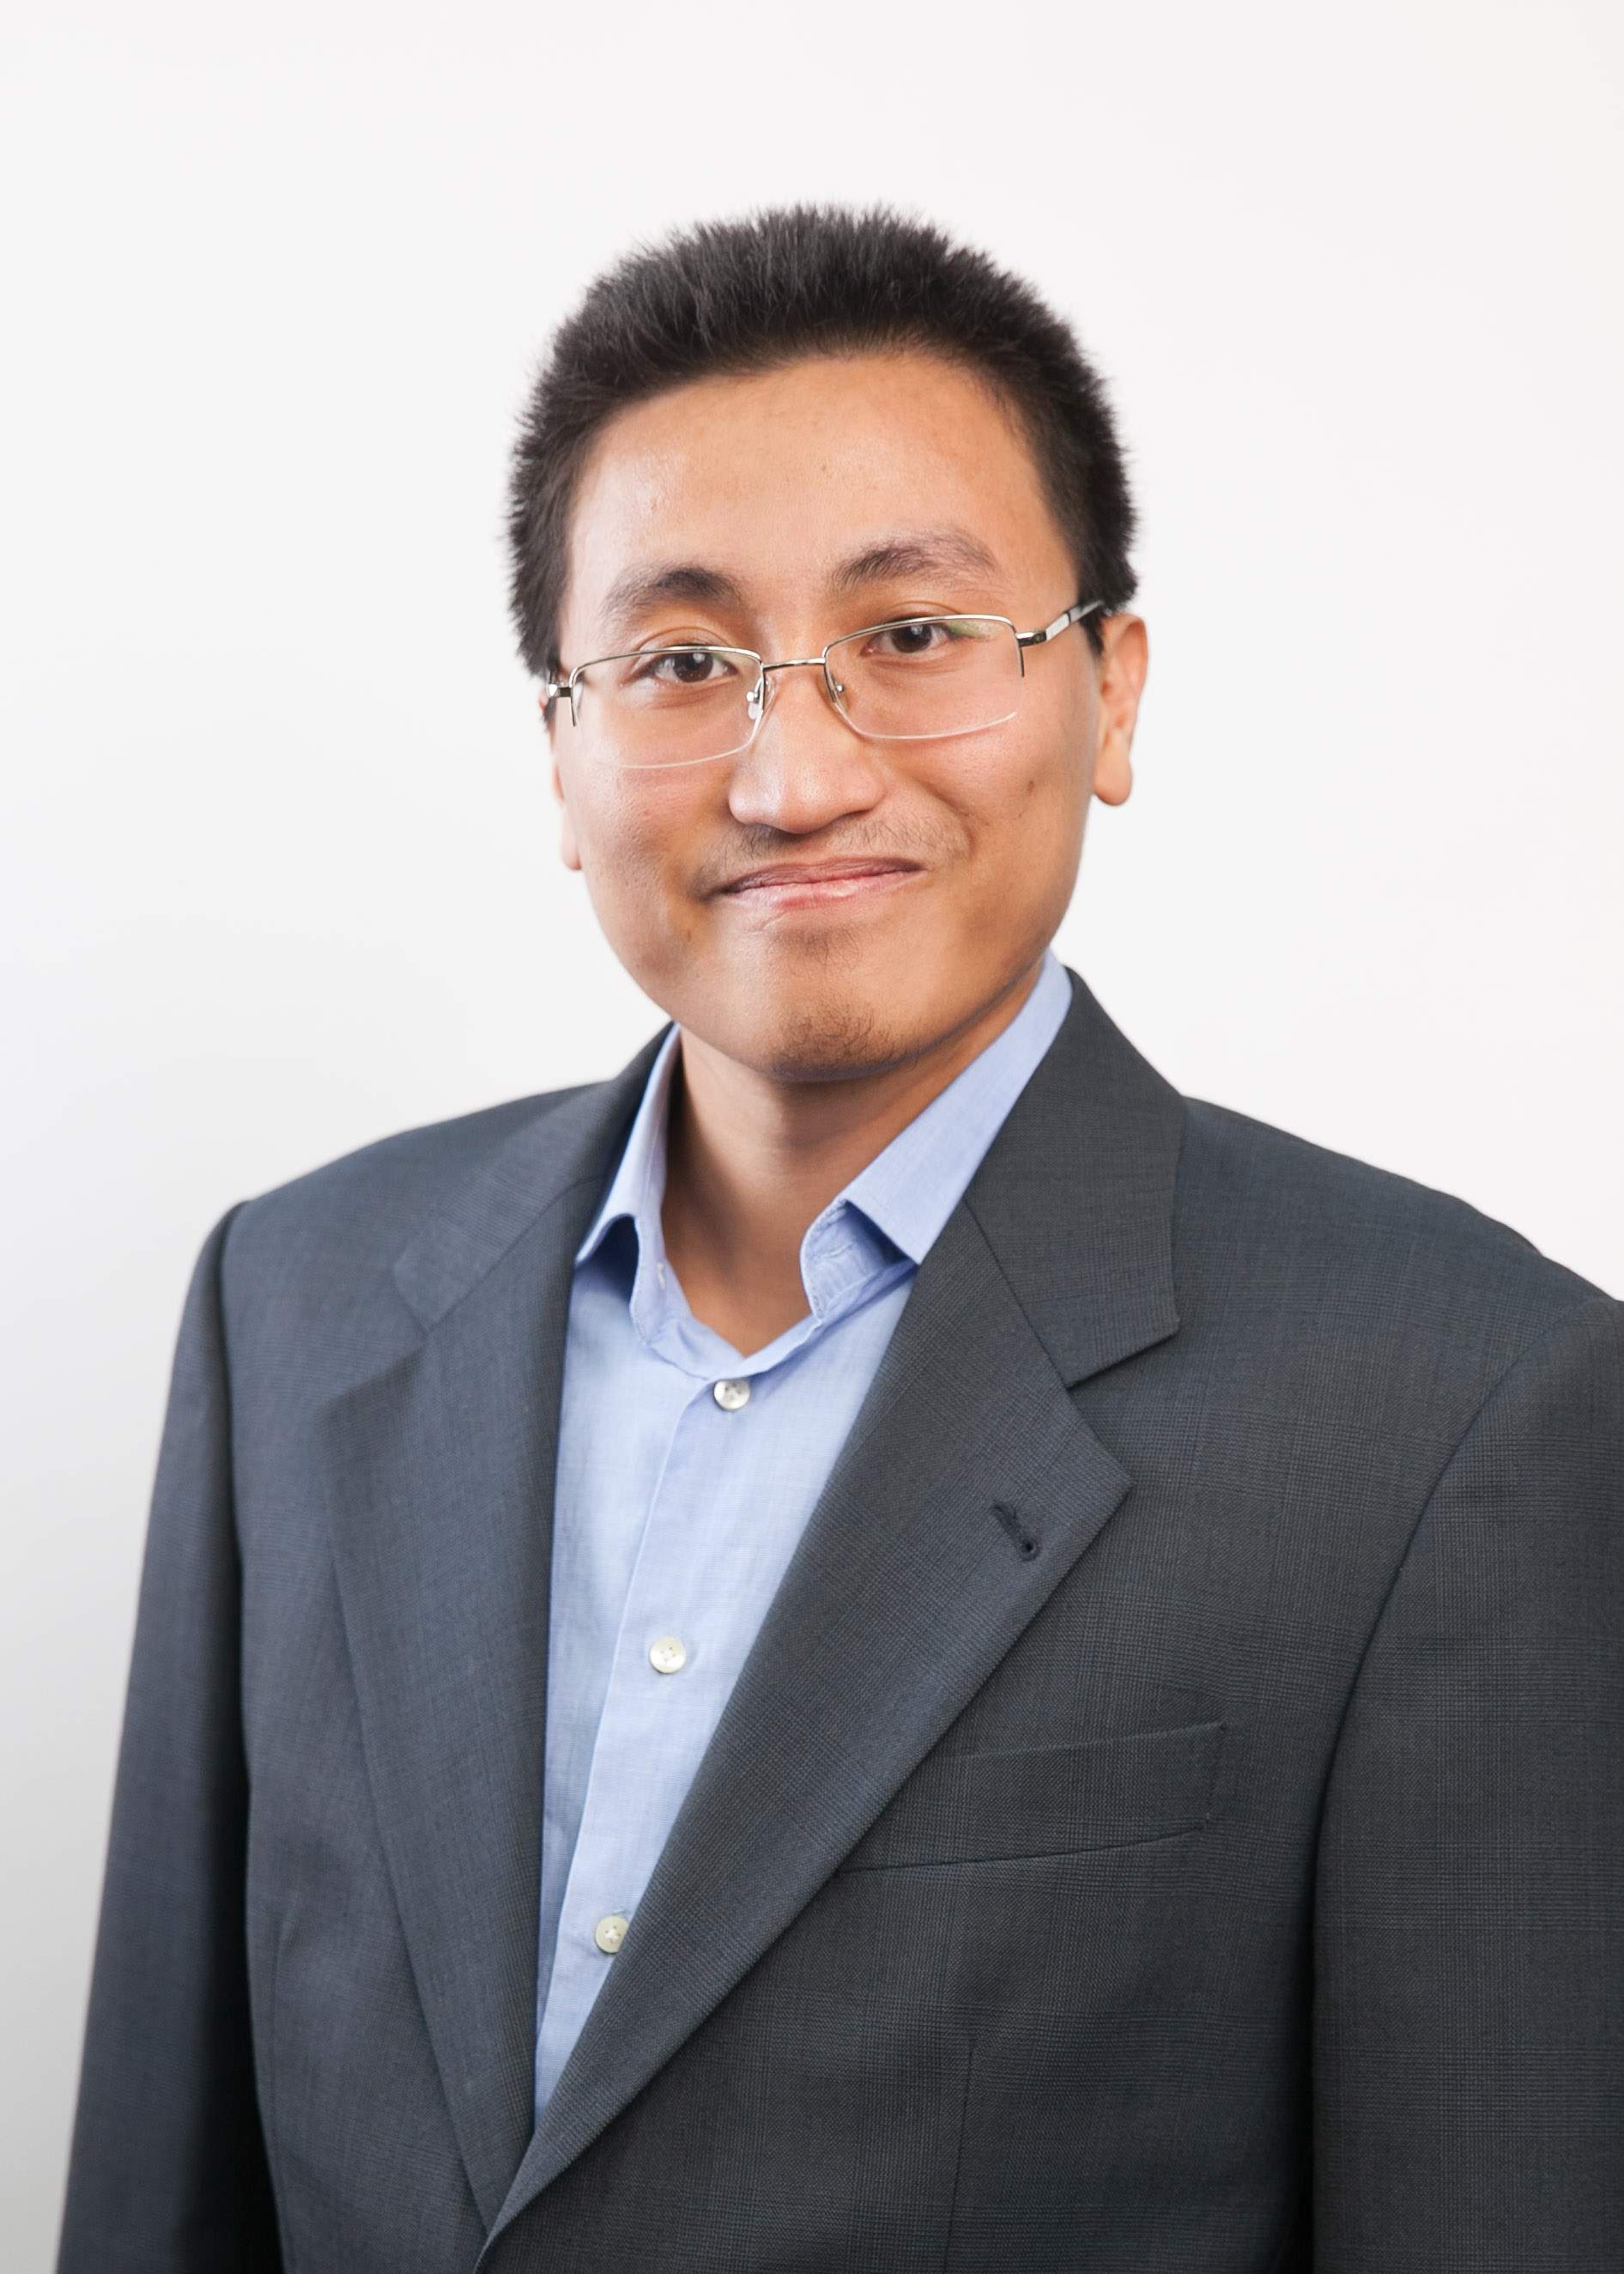
\includegraphics[width=2.75cm]{cv/photo}
\end{minipage}

% Print the footer with 3 arguments(<left>, <center>, <right>)
% Leave any of these blank if they are not needed
\makecvfooter
  {\today}
  {Nguyen Chanh Dat~~~·~~~Curriculum Vitae}
  {\thepage}


%-------------------------------------------------------------------------------
%	CV/RESUME CONTENT
%	Each section is imported separately, open each file in turn to modify content
%-------------------------------------------------------------------------------
%-------------------------------------------------------------------------------
%	SECTION TITLE
%-------------------------------------------------------------------------------
\cvsection{Education}


%-------------------------------------------------------------------------------
%	CONTENT
%-------------------------------------------------------------------------------
\begin{cventries}

%---------------------------------------------------------
\cventry
{B.Sc. in Mechanical Engineering} % Degree
{The Lucerne University of Applied Sciences and Arts} % Institution
{Luzern, Switzerland} % Location
{2016 - 2020} % Date(s)
{
	\begin{cvitems} % Description(s) bullet points
		\item {\textbf{Major}: Product Design and Mechatronics}
		\item {\textbf{Project}: Collaborated to conceptualize and realize an autonomous, all-terrain robot, transporting cargo (based on Mars Rover design).}
		\item {\textbf{Bachelor thesis}: Develop a bioreactor as part of life supporting system for a moon habitat - \newline \textit{Industry partner}: \mbox{SwissSpaceCenter} (SSC) \& European Space Agency (ESA - Biotesc: Space biology/medicine group) (2019)}
	\end{cvitems}
}


%---------------------------------------------------------
%  \cventry
%    {B.Sc. in Mechanical Engineering} % Degree
%    {ETH Zürich(Swiss Federal Institute of Technology in Zurich)} % Institution
%    {Zurich, Switzerland} % Location
%    {} % Date(s)
%    {
%      \begin{cvitems} % Description(s) bullet points
%        \item {Teaching Assistant: Introduction to Fortran Programming}
%        \item {Programming Assistant: Data analysis with Python and PostgreSQL}
%      \end{cvitems}
%    }

%---------------------------------------------------------
  \cventry
    {Highschool} % Degree
    {KSR (Kantonsschule Reussbühl)} % Institution
    {Luzern, Switzerland} % Location
    {} % Date(s)
    {
      \begin{cvitems} % Description(s) bullet points
        \item {Major: Mathematics and physics}
      \end{cvitems}
    }

%---------------------------------------------------------
\end{cventries}

%-------------------------------------------------------------------------------
%	SECTION TITLE
%-------------------------------------------------------------------------------
\cvsection{Skills}


%-------------------------------------------------------------------------------
%	CONTENT
%-------------------------------------------------------------------------------
\begin{cvskills}

%---------------------------------------------------------
  \cvskill
    {Engineering Tools} % Category
    {\textbf{CAD}: (UNI NX, Solidworks, Autodesk Inventor); MatLAB, Mathematica,\newline \textbf{CFD}: OpenFOAM
    \newline \textbf{SPS}: TwinCAT3, Selectron CAP1131
	\newline \textbf{FEM}: Ansys (statics)} % Skills

%---------------------------------------------------------
  \cvskill
    {Manufacturing Tools} % Category
    {\textbf{3D Print/CNC}: Skeinforge, G-Code;} % Skills

%---------------------------------------------------------
  \cvskill
    {Programming} % Category
    {R/Python, C/C++, Fortran, Ruby, PHP, LaTeX \newline% Skills 
    \textbf{Languages}: Python, C/C++, Fortran, Ruby, LaTeX, 
    	\newline \textbf{Database}: MySQL/PostgreSQL,
    	\newline \textbf{Version Control}: Git} % Skills

%---------------------------------------------------------
%  \cvskill
%    {Web} % Category
%    {Ruby on Rails, SQL (MySQL/PostgreSQL)} % Skills

%---------------------------------------------------------
  \cvskill
    {Languages} % Category
    {Vietnamese (mother tounge), German (fluent), English (fluent), Italian (B1)} % Skills

%---------------------------------------------------------
\end{cvskills}

%-------------------------------------------------------------------------------
%	SECTION TITLE
%-------------------------------------------------------------------------------
\cvsection{Experience}


%-------------------------------------------------------------------------------
%	CONTENT
%-------------------------------------------------------------------------------
\begin{cventries}
	
%---------------------------------------------------------
\cventry
{Internship in Product Management and D\&D} % Job title
{Bühler AG} % Organization
{Uzwil, Switzerland} % Location
{Feb. 2019 - now} % Date(s)
{
  \begin{cvitems} % Description(s) of tasks/responsibilities
    \item {Market analyse: Benchmarking various product families in Business Component (BC)'s portfolio (i.e. filters, airlocks, pipe diverters) against competitors (on market share, and define optimal manufacturing cost/sales prices in Navigator), to maximise the margin-potential.}
    \item {CAQ: Analyse statistics of installation and customer complains, to identify the problem hotspots for further development opportunities.}
    \item {Support international Sales Dept. with creating/configurating quotations in Navigator, and offering technical clarifications (via standard sheets or in contact with Lifecycle-managers).}
    \item {Managing Design-to-Cost projects, to further reduce manufacturing cost (i.e. diverters).}
    \item {Analyse and improve the filter porfolio on explosion-protection as well as dust emission to satisfy the conformity requirements (ATEX/IEC-Ex, AEx-NFPA68, etc.) and components conformity requirements for food safety (FDA).}
    \item {Create safety analysis (SANA) for the conformity certification of the hopper filter LCCB.}
    \item {Building testing rigs, to test prototypes, specimen of suppliers: EPDM membranes, bearing rings, filter control units.}
    \item {Project management: Collaborate with various production sites (BZAM, BCHI, BBAN, etc.) to standardize the universal motor, and support roll-out airlock (MPSx), cyclone (MGXx) and filter (MVRx) on SIMBA}
  \end{cvitems}
}

%---------------------------------------------------------
\cventry
  {Helper} % Job title
  {Swiss Steel AG} % Organization
  {Emmenbrücke, Switzerland} % Location
  {Jul. 2018 - Sep. 2018} % Date(s)
  {
    \begin{cvitems} % Description(s) of tasks/responsibilities
      \item {Support the annual revision of steel works (reservoirs, hydraulics crane systems).}
      \item {Carry out maintenance work at various parts of the production plant (of construction steel beams)}
    \end{cvitems}
} 

%---------------------------------------------------------
\cventry
{Engineering Internship} % Job title
{Hartmetall Estech AG} % Organization
{Hitzkirch, Switzerland} % Location
{Jul. 2017 - Sep. 2017} % Date(s)
{
	\begin{cvitems} % Description(s) of tasks/responsibilities
		\item {Assist in production hall}
    \item {Prepare quality control probes, before and after sinstering process.}
	\end{cvitems}
}

%---------------------------------------------------------
\cventry
  {Partime worker} % Job title
  {Zimmermann Technik AG} % Organization
  {Luzern, Switzerland} % Location
  {} % Date(s)
  {
    \begin{cvitems} % Description(s) of tasks/responsibilities
      \item {Assemble and test magnet coils and various electronics systems/control cabinets.}
    \end{cvitems}
  } 


%---------------------------------------------------------
  \cventry
    {SysAdmin - Operating Manager} % Job title
    {SPOD - VSETH} % Organization
    {Switzerland} % Location
    {Dec. 2013 - 2016} % Date(s)
    {
      \begin{cvitems} % Description(s) of tasks/responsibilities
        \item {Debugging a legacy Ruby on Rails application and developing a new replacement}
        \item {ICT-support for Windows, Mac and Linux systems}
      \end{cvitems}
    }

%---------------------------------------------------------
  \cventry
    {Engineering Internship} % Job title
    {Reiden Technik AG} % Organization
    {Reiden, Switzerland} % Location
    {Jan. 2013 - Apr. 2013} % Date(s)
    {
      \begin{cvitems} % Description(s) of tasks/responsibilities
        \item {Assemble the combined milling and lathing CNC machines: RX-Serie (RX-10, RX14, and RX-18)}
      \end{cvitems}
    }

%---------------------------------------------------------

\end{cventries}

%-------------------------------------------------------------------------------
%	SECTION TITLE
%-------------------------------------------------------------------------------
\cvsection{Extracurricular Activity}


%-------------------------------------------------------------------------------
%	CONTENT
%-------------------------------------------------------------------------------
\begin{cventries}

%---------------------------------------------------------
\cventry
{Member} % Affiliation/role
{KCL - Kanu Club Luzern} % Organization/group
{Luzern, Switzerland} % Location
{current} % Date(s)
{
  \begin{cvitems} % Description(s) of experience/contributions/knowledge
    \item {Canadian canoe/kayaking}
  \end{cvitems}
}

%---------------------------------------------------------
  \cventry
{Teaching Assisstant} % Affiliation/role
{Scientifica, ETH Zurich and University of Zurich} % Organization/group
{Zurich, Switzerland} % Location
{2015} % Date(s)
{
  \begin{cvitems} % Description(s) of experience/contributions/knowledge
    \item {Supervise 4 groups of 10 to 15 children, aged from 10 to 14, for the workshop "Introduction to Robotics, with Thymio II".}
  \end{cvitems}
}

%---------------------------------------------------------
  \cventry
{Assisstant} % Affiliation/role
{TheAlternative.ch, [project 21]} % Organization/group
{Zurich, Switzerland} % Location
{2014 - 2015} % Date(s)
{
  \begin{cvitems} % Description(s) of experience/contributions/knowledge
    \item {Helper and Troublershooter at various Linux Installation Day events.}
  \end{cvitems}
}

%---------------------------------------------------------
  \cventry
{Member} % Affiliation/role
{SCI Switzerland (Service Civil International)} % Organization/group
{Switzerland} % Location
{2010 - 2014} % Date(s)
{
  \begin{cvitems} % Description(s) of experience/contributions/knowledge
    \item {Help distributing used clothes and food for homeless people around St. Pauli, Hamburg at Alimaus St.Ansgar e.V.}
  \end{cvitems}
}

\end{cventries}

%%-------------------------------------------------------------------------------
%	SECTION TITLE
%-------------------------------------------------------------------------------
\cvsection{Honors \& Awards}


%-------------------------------------------------------------------------------
%	SUBSECTION TITLE
%-------------------------------------------------------------------------------
\cvsubsection{International}


%-------------------------------------------------------------------------------
%	CONTENT
%-------------------------------------------------------------------------------
\begin{cvhonors}

%---------------------------------------------------------
  \cvhonor
    {Finalist} % Award
    {DEFCON 22nd CTF Hacking Competition World Final} % Event
    {Las Vegas, U.S.A} % Location
    {2014} % Date(s)

%---------------------------------------------------------
  \cvhonor
    {Finalist} % Award
    {DEFCON 21st CTF Hacking Competition World Final} % Event
    {Las Vegas, U.S.A} % Location
    {2013} % Date(s)

%---------------------------------------------------------
  \cvhonor
    {Finalist} % Award
    {DEFCON 19th CTF Hacking Competition World Final} % Event
    {Las Vegas, U.S.A} % Location
    {2011} % Date(s)

%---------------------------------------------------------
  \cvhonor
    {6th Place} % Award
    {SECUINSIDE Hacking Competition World Final} % Event
    {Seoul, S.Korea} % Location
    {2012} % Date(s)

%---------------------------------------------------------
\end{cvhonors}


%-------------------------------------------------------------------------------
%	SUBSECTION TITLE
%-------------------------------------------------------------------------------
\cvsubsection{Domestic}


%-------------------------------------------------------------------------------
%	CONTENT
%-------------------------------------------------------------------------------
\begin{cvhonors}

%---------------------------------------------------------
  \cvhonor
    {3rd Place} % Award
    {WITHCON Hacking Competition Final} % Event
    {Seoul, S.Korea} % Location
    {2015} % Date(s)

%---------------------------------------------------------
  \cvhonor
    {Silver Prize} % Award
    {KISA HDCON Hacking Competition Final} % Event
    {Seoul, S.Korea} % Location
    {2013} % Date(s)

%---------------------------------------------------------
  \cvhonor
    {2nd Award} % Award
    {HUST Hacking Festival} % Event
    {S.Korea} % Location
    {2013} % Date(s)

%---------------------------------------------------------
  \cvhonor
    {3rd Award} % Award
    {HUST Hacking Festival} % Event
    {S.Korea} % Location
    {2010} % Date(s)

%---------------------------------------------------------
  \cvhonor
    {3rd Award} % Award
    {Holyshield 3rd Hacking Festival} % Event
    {S.Korea} % Location
    {2012} % Date(s)

%---------------------------------------------------------
  \cvhonor
    {2nd Award} % Award
    {Holyshield 3rd Hacking Festival} % Event
    {S.Korea} % Location
    {2011} % Date(s)

%---------------------------------------------------------
  \cvhonor
    {5th Place} % Award
    {PADOCON Hacking Competition Final} % Event
    {Seoul, S.Korea} % Location
    {2011} % Date(s)

%---------------------------------------------------------
\end{cvhonors}

%%-------------------------------------------------------------------------------
%	SECTION TITLE
%-------------------------------------------------------------------------------
\cvsection{(Personal) Projects}


%-------------------------------------------------------------------------------
%	CONTENT
%-------------------------------------------------------------------------------
\begin{cventries}

  %---------------------------------------------------------
  \cventry
  {} % Role
  {Amateur radio (HAM)} % Event
  {} % Location
  {} % Date(s)
  {\vspace{-12pt}
    \begin{cvitems} % Description(s)
      \item {HB3 - License}
      \item {Member of amateur radio club of HSLU: HB9HSLU}
    \end{cvitems}
  }

%---------------------------------------------------------
\cventry
{} % Role
{Develop a doctor office management application (ongoing)} % Event
{} % Location
{} % Date(s)
{\vspace{-12pt}
	\begin{cvitems} % Description(s)
		\item {Collaboration with Dr. med. Khanh Tran (Dagmersellen)}
		\item {Retrieve patient and his/her insurance info from HIN(\textit{Health Info Net AG})}
		\item {Maintain an up-to-date medicine list (from Federal Office of Public Health Switzerland, BaG)}
		\item {Generate bills and send them to insurance companies (using MediData.ch service)}
	\end{cvitems}
}

%---------------------------------------------------------
\cventry
{} % Role
{Build a weather station (complete)} % Event
{} % Location
{} % Date(s)
{\vspace{-12pt}
	\begin{cvitems} % Description(s)
		\item {Coming in 2 versions: Handheld measure device and stationary measure station}
		\item {Measuring temperature, humidity (using DHT22) and pressure (using BMP085)}
		\item {Stationary station: 2 Arduinos connect with each other over 2.4 Ghz frequency using XBee 1mW Wire Antenna - Series 1}
	\end{cvitems}
}

%---------------------------------------------------------
  \cventry
    {} % Role
    {Build a hexacopter (complete)} % Event
    {} % Location
    {} % Date(s)
    {\vspace{-12pt}
      \begin{cvitems} % Description(s)
        \item {Payload: $ \sim 700g$}
        \item {Controller: Paris SIRIUS with 3 axis gyroscope and GPS receiver}
      \end{cvitems}
    }

%---------------------------------------------------------
  \cventry
    {} % Role
    {Design and build a tabletop CNC-Router (complete)} % Event
    {} % Location
    {} % Date(s)
    {\vspace{-12pt}
      \begin{cvitems} % Description(s)
        \item {2.5D-machining/milling}
        \item {Material: polystyrene, wood, MDF, Plexi glas, Plastic PVC, etc.}
      \end{cvitems}
    }

%---------------------------------------------------------
\end{cventries}

%-------------------------------------------------------------------------------
%	SECTION TITLE
%-------------------------------------------------------------------------------
\cvsection{Writing}


%-------------------------------------------------------------------------------
%	CONTENT
%-------------------------------------------------------------------------------
\begin{cventries}

%---------------------------------------------------------
  \cventry
    {Founder \& Writer} % Role
    {A Guide for beginners to Arduino and wireless technology (XBee)} % Title
    {Personal Blog} % Location
    {2010 - 2013} % Date(s)
    {
      \begin{cvitems} % Description(s)
        \item {Various interessting code snippets and Do-It-Yourself tutorials (Weather tracking system, Hexacopter, tabletop CNC router)}
      \end{cvitems}
    }

%---------------------------------------------------------

\end{cventries}

%-------------------------------------------------------------------------------
%	SECTION TITLE
%-------------------------------------------------------------------------------
\cvsection{Program Committees}


%-------------------------------------------------------------------------------
%	CONTENT
%-------------------------------------------------------------------------------
\begin{cvhonors}

%---------------------------------------------------------
  \cvhonor
    {Resprenstative} % Position
    {Activity Fair} % Committee
    {Switzerland} % Location
    {2014, 2015} % Date(s)

%---------------------------------------------------------
  \cvhonor
    {Staff} % Position
    {Scientifica Event} % Committee
    {Switzerland} % Location
    {2015} % Date(s)

%---------------------------------------------------------
\end{cvhonors}



%-------------------------------------------------------------------------------
\end{document}
